%%%%%%%%%%%%%%%%%%%%%%%%%%%%%%%%%%%%%%%%%%%%%%%%%%%%%%%%%%%%%%%%%%%%
%% I, the copyright holder of this work, release this work into the
%% public domain. This applies worldwide. In some countries this may
%% not be legally possible; if so: I grant anyone the right to use
%% this work for any purpose, without any conditions, unless such
%% conditions are required by law.
%%%%%%%%%%%%%%%%%%%%%%%%%%%%%%%%%%%%%%%%%%%%%%%%%%%%%%%%%%%%%%%%%%%%

\documentclass{beamer}
% Compile from slides/ (editor or: latexmk -pdf -cd slides/ped-pdflatex.tex).
% Theme sty is symlinked here; fibeamer/ and resources/ live one level up.
\usetheme[faculty=ped,basePath=../fibeamer,logo=../fibeamer/logo/mu/Logo-UC-3.png]{fibeamer}
\graphicspath{{../resources/}}

\usepackage{algorithm}
\usepackage{algpseudocode}

\usepackage[utf8]{inputenc}
\usepackage[
  main=english, %% By using `czech` or `slovak` as the main locale
                %% instead of `english`, you can typeset the
                %% presentation in either Czech or Slovak,
                %% respectively.
  czech, slovak %% The additional keys allow foreign texts to be
]{babel}        %% typeset as follows:
%%
%%   \begin{otherlanguage}{czech}   ... \end{otherlanguage}
%%   \begin{otherlanguage}{slovak}  ... \end{otherlanguage}
%%
%% These macros specify information about the presentation
\title{IIC1103 - Introducción a la Programación} %% that will be typeset on the
\subtitle{Semestre II-2026} %% title page.
\author{Andreina Cota Vidaurre}
%% These additional packages are used within the document:
\usepackage{ragged2e}  % `\justifying` text
\usepackage{booktabs}  % Tables
\usepackage{tabularx}
\usepackage{tikz}      % Diagrams
\usetikzlibrary{calc, shapes, backgrounds}
\usetikzlibrary{positioning, arrows.meta, shadows.blur, shapes.geometric}
\usepackage{amsmath, amssymb}
\usepackage{url}       % `\url`s
\usepackage{listings}  % Code listings
\usepackage{graphicx}
\usepackage{amsmath}
\usepackage[T1]{fontenc}
\usepackage{xcolor}
\usepackage{pifont}
\usepackage{csquotes}
\usepackage{hyperref}
% \usepackage{adjustbox}


% Definicion de pseudocodigo en espaniol
\lstdefinelanguage{PseudocodigoES}{
    morekeywords={INICIO,FIN,PARA,HACER,SI,ENTONCES,FIN_SI,FIN_PARA,IMPRIMIR},
    sensitive=true,
    morecomment=[l]{//},
    morestring=[b]"
}

% Definicion de pseudocodigo en ingles
\lstdefinelanguage{PseudocodeEN}{
    morekeywords={BEGIN,END,FOR,DO,IF,THEN,END_IF,END_FOR,PRINT},
    sensitive=true,
    morecomment=[l]{//},
    morestring=[b]"
}

\lstset{
    basicstyle=\ttfamily\small,
    keywordstyle=\bfseries,
    columns=fullflexible,
    keepspaces=true,
    showstringspaces=false,
    frame=single,
    xleftmargin=0em,
    framexleftmargin=0em,
    framesep=2pt,
    gobble=4,
    resetmargins=true,
    aboveskip=0pt,
    belowskip=0pt
}

\lstdefinestyle{pythonstyle}{
    language=Python,
    basicstyle=\ttfamily\small,
    keywordstyle=\bfseries,
    commentstyle=\itshape,
    stringstyle=\ttfamily,
    showstringspaces=false,
    columns=fullflexible,
    keepspaces=true,
    frame=single,
    breaklines=true,
    xleftmargin=0em,
    framexleftmargin=0em,
    framesep=2pt,
    aboveskip=0pt,
    belowskip=0pt,
    gobble=4,
    resetmargins=true,
    emph={print,input,int,float,str,bool,len,range},
    emphstyle=\bfseries
}

\lstset{style=pythonstyle}

% Estilos del diagrama
\tikzstyle{iniciofin} = [
    ellipse,
    minimum width=2.5cm,
    minimum height=1cm,
    text centered,
    draw=black,
    fill=blue!25
]

\tikzstyle{proceso} = [
    rectangle,
    rounded corners,
    minimum width=3cm,
    minimum height=1cm,
    text centered,
    draw=black,
    fill=cyan!20
]

\tikzstyle{decision} = [
    diamond,
    aspect=2,
    text centered,
    draw=black,
    fill=yellow!35
]

\tikzstyle{flecha} = [
    thick,
    ->,
    >=Stealth
]

% \definecolor{green_python}{HTML}{52A736}

% \newcolumntype{Y}{>{\raggedright\arraybackslash}X}

\frenchspacing
\begin{document}
  \shorthandoff{-}
  \frame[c]{\maketitle}

% \begin{darkframes}

    \begin{frame}{Contenido}
        \begin{itemize}
            \item \hyperlink{introduccion}{Introducción al curso}
            \item \hyperlink{competencias}{Competencias y Aprendizajes Esperados}
            \item \hyperlink{contenidos}{Contenidos del curso}
            \item \hyperlink{metodologia}{Metodología de Trabajo}
            \item \hyperlink{contacto}{Contacto}
            \item \hyperlink{evaluacion}{Sistema de Evaluación}
            \item \hyperlink{normativa}{Normativa del Curso}
            \item \hyperlink{integridad-academica}{Integridad Académica}
            \item \hyperlink{calendario}{Calendario de actividades}
            \item \hyperlink{bibliografia}{Bibliografía}
        \end{itemize}
    \end{frame}

    \begin{frame}{Contacto}
        \begin{itemize}
            \item Profesora: Andreina Cota Vidaurre, acota@uc.cl - Materia, situaciones especiales.
            \item Ayudante de Cátedra: Victoria Guzman, vguzman1@estudiante.uc.cl - Materia, notas de participación, ayuda en aula.
            \item Ayudante de Bienestar: Josefa Viveros, jviverosa@estudiante.uc.cl - Ayuda en bienestar, situaciones especiales.
            \item Coordinación: Santiago de la Carrera Bezanilla, iic1103@uc.cl - Coordinación, logística, justificativo DIPRE.
        \end{itemize}
    \end{frame}

    \begin{frame}[label=introduccion]{Introducción al curso}
        \begin{itemize}
            \item IIC1103 - Introducción a la Programación
            \item Sección 12, martes y jueves 08:20 - 09:30
            \item Curso de 10 créditos, sin requisitos previos
            \item Objetivo: Entregar las herramientas fundamentales para transformar 
            ideas en soluciones computacionales, mediante el desarrollo del \textbf{pensamiento algorítmico} 
            y la \textbf{programación orientada a objetos}
        \end{itemize}
    \end{frame}

    \begin{frame}{¿Por qué programar?}
        \begin{quote}
            \enquote{Todo el mundo debería aprender a programar un ordenador, porque esto te ayuda a pensar.}
            \hfill \textbf{Steve Jobs}
        \end{quote}
        \begin{itemize}
            \item Programar es, en esencia, dar instrucciones precisas y ordenadas para que alguien o algo resuelva un problema.
            \item Aprender a programar es aprender a descomponer problemas complejos en pasos simples y ejecutables.
            \item La forma de pensar que menciona Jobs es el \textbf{pensamiento algorítmico}. Habilidad de descomponer un problema
            en una secuencia de pasos simples, ordenados y ejecutables.
        \end{itemize}
    \end{frame}

    \begin{frame}{Algoritmo}
        \begin{figure}
            \centering
            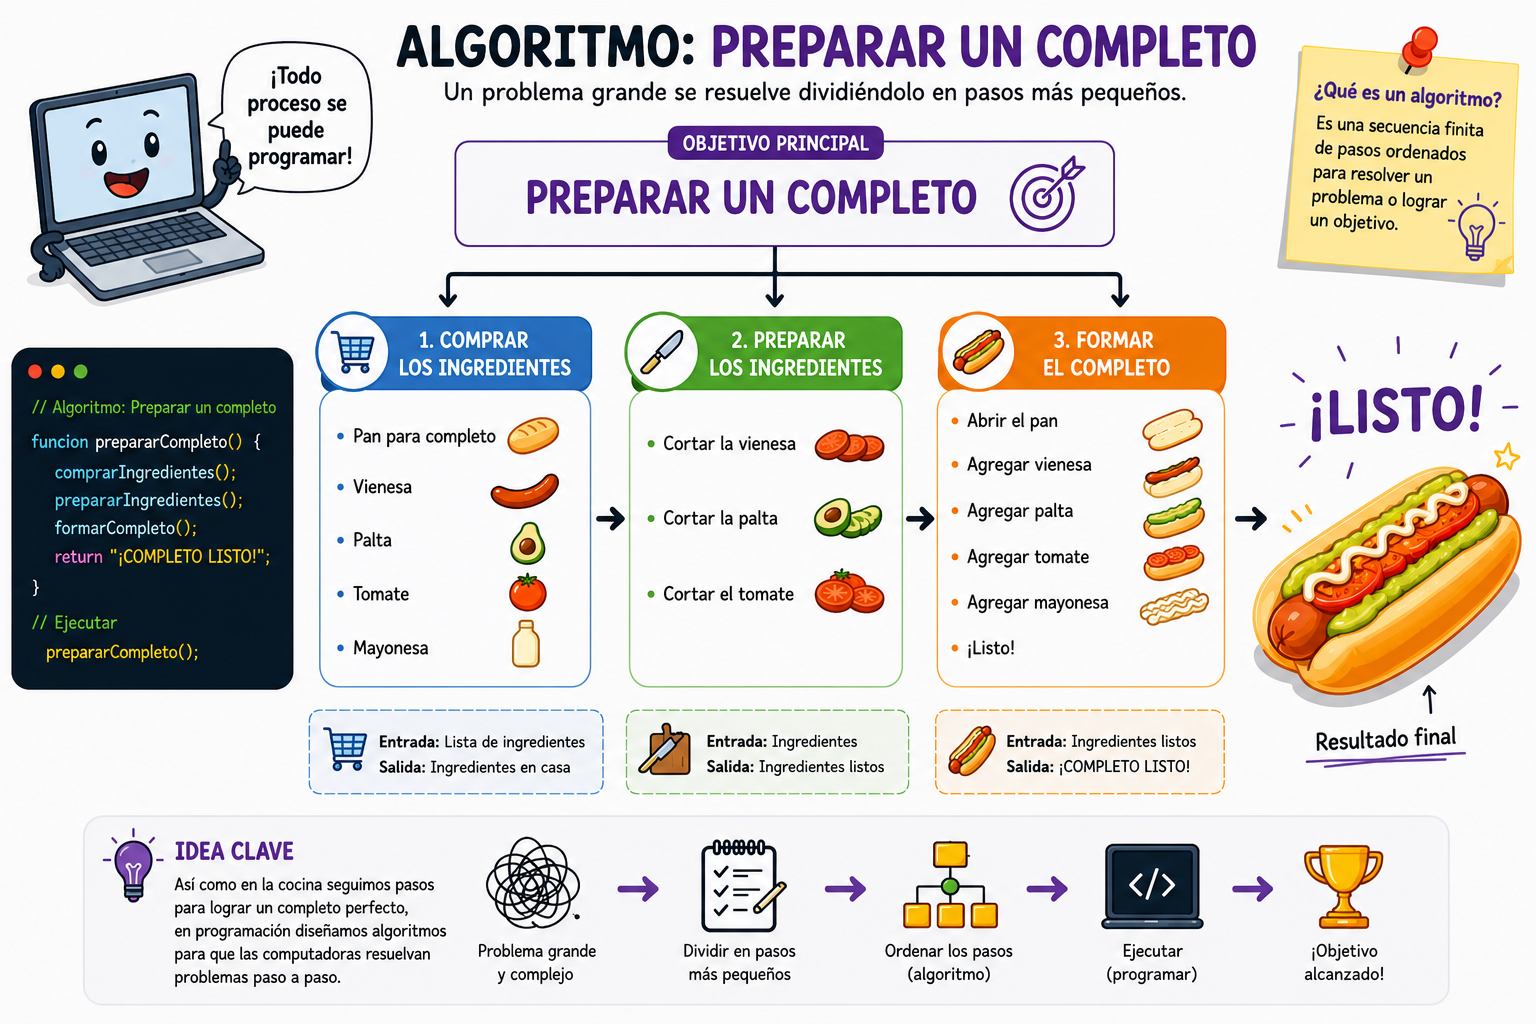
\includegraphics[width=\linewidth]{algoritmo_completo.png}
        \end{figure}
    \end{frame}

    \begin{frame}[label=competencias]{Competencias y Aprendizajes Esperados}
        \begin{itemize}
            \item Pensar algorítmicamente: Identificar problemas, descomponerlos en pasos simples y diseñar soluciones antes 
            de escribir código.
            \item Dominar las herramientas de Python: Usar variables, estructuras de control, funciones, strings y 
            listas para construir soluciones funcionales.
            \item Programar con un enfoque profesional: Aplicar programación orientada a objetos, y escribir/depurar programas propios 
            de forma autónoma.
        \end{itemize}
    \end{frame}

    \begin{frame}{¿Por qué estas competencias importan?}
        \begin{itemize}
            \item Pensamiento algorítmico $\rightarrow$ resolución de problemas en general: La lógica de descomponer un problema en 
            pasos es transversal a cualquier área.
            \item Automatización $\rightarrow$ eficiencia: La programación permite automatizar tareas repetitivas, aumentando la productividad.
            \item Autonomía técnica: Ser capaz de escribir y depurar tus propios programas, sin depender de otros.
        \end{itemize}
    \end{frame}

    % \begin{frame}[label=contenidos]{Contenidos del curso}
    %     \begin{enumerate}
    %         \item Introduccion a los algoritmos
    %         \item El lenguaje de programación Python
    %         \item Variables y expresiones
    %         \item Control de flujo
    %         \item Funciones
    %         \item Strings
    %         \item Listas
    %         \item Recursión
    %         \item Archivos
    %         \item Programación orientada a objetos
    %         \item Ordenamiento
    %     \end{enumerate}
    % \end{frame}

    \begin{frame}[label=contenidos]{Etapa 1: Fundamentos de programación}

        \begin{block}{1. Introducción a los algoritmos}
        Comprender qué es un algoritmo.
        \end{block}
        
        \begin{block}{2. El lenguaje de programación Python}
        Conocer la sintaxis básica de Python y ejecutar instrucciones.
        \end{block}
        
        \begin{block}{3. Variables y expresiones}
        Trabajar con datos, variables, operaciones, comparaciones, entrada y salida de datos.
        \end{block}

        \begin{block}{4. Control de flujo}
            Iteraciones mediante condicionales y ciclos.
        \end{block}
        
    \end{frame}

    % \begin{frame}{Etapa 1: Fundamentos de programación}
        
    %     \begin{block}{4. Control de flujo}
    %     Construir programas con decisiones e iteraciones mediante
    %     condicionales y ciclos.
    %     \end{block}
        
    % \end{frame}

    \begin{frame}{Etapa 2: Organizar y procesar información}

        \begin{block}{5. Funciones}
        Dividir un programa en partes reutilizables mediante funciones,
        parámetros, retorno y variables locales.
        \end{block}
        
        \begin{block}{6. Strings}
        Procesar texto, recorrer caracteres, buscar información,
        extraer partes y utilizar métodos de strings.
        \end{block}
        
        \begin{block}{7. Listas}
        Almacenar colecciones de elementos, recorrerlas, modificarlas
        y trabajar con listas simples y listas anidadas.
        \end{block}
        
    \end{frame}

    \begin{frame}{Etapa 3: Resolver problemas y almacenar información}

        \begin{block}{8. Recursión}
        Resolver problemas mediante funciones que se llaman a si mismas,
        utilizando un caso base y un caso recursivo.
        \end{block}
        
        \begin{block}{9. Archivos}
        Leer, procesar y escribir información almacenada en archivos
        de texto y archivos CSV.
        \end{block}
        
    \end{frame}

    \begin{frame}{Etapa 4: Construcción de programas más complejos}

        \begin{block}{10. Programación orientada a objetos}
        Representar entidades mediante clases, objetos, atributos,
        constructores y métodos.
        \end{block}
        
        \begin{block}{11. Ordenamiento}
        Ordenar datos utilizando funciones de Python y comprender
        la idea de los algoritmos de ordenamiento.
        \end{block}
        
    \end{frame}

    \begin{frame}{¿Cómo avanzaremos?}

        \centering
        
        Algoritmos y Python
        
        $\downarrow$
        
        Variables y expresiones
        
        $\downarrow$
        
        Control de flujo
        
        $\downarrow$
        
        Funciones
        
        $\downarrow$
        
        Strings y listas
        
        $\downarrow$
        
        Recursión y archivos
        
        $\downarrow$
        
        Clases, objetos y ordenamiento
        
    \end{frame}

    \begin{frame}[label=metodologia]{Metodología de trabajo}
        \begin{itemize}
            \item Clases de cátedra: 2 módulos semanales
            \item Salas de Ayudantía Presencial (SAP): 2 módulos semanales, con ayudantes para resolver dudas de 
            ejercicios, tareas y material de estudio. Se puede asistir en cualquier horario disponible.
            \item Trabajo autónomo: Se espera un promedio de 6 horas semanales fuera de clase, dedicadas a practicar,
            avanzar en tareas y repasar contenidos.
        \end{itemize}
    \end{frame}

    \begin{frame}{Canal de comunicación y plataforma de trabajo}
        \begin{itemize}
            \item Todos los avisos oficiales del curso se publican en: \href{https://cursos.canvas.uc.cl}{Canvas}
            \raisebox{-0.35\height}{
\includegraphics[height=1.1em]{canvas.png}}
            \item Es responsabilidad de cada estudiante revisar Canvas regularmente para mantenerse informado sobre
            las actividades del curso.
            \item La plataforma para realizar las tareas y ejercicios es: \href{https://www.clearn.cl/}{Clearn}
            \raisebox{-0.35\height}{
\includegraphics[height=1.1em]{clearn_full.png}}
        \end{itemize}
    \end{frame}

    \begin{frame}[label=contacto]{Contacto}
        \begin{itemize}
            \item Profesora: Andreina Cota Vidaurre, acota@uc.cl - Materia, situaciones especiales.
            \item Ayudante de Cátedra: Victoria Guzman, vguzman1@estudiante.uc.cl - Materia, notas de participación, ayuda en aula.
            \item Ayudante de Bienestar: Josefa Viveros, jviverosa@estudiante.uc.cl - Ayuda en bienestar, situaciones especiales.
            \item Coordinación: Santiago de la Carrera Bezanilla, iic1103@uc.cl - Coordinación, logística, justificativo DIPRE.
        \end{itemize}
    \end{frame}

    \begin{frame}[label=evaluacion]{Sistema de Evaluación}

        Busca medir progresivamente la capacidad de comprender problemas, diseñar soluciones algorítmicas e
        implementarlas correctamente en Python.

        \begin{itemize}
            \item Evaluaciones individuales de contenidos.
            \item Tareas de aplicación y práctica.
            \item Participación en las actividades del curso.
            \item Uso responsable de herramientas de inteligencia artificial.
        \end{itemize}
    \end{frame}

    \begin{frame}{Nota Final}

        \begin{columns}[T]
        
        \begin{column}{0.48\textwidth}
        \begin{block}{Evaluaciones principales}
        \begin{itemize}
            \item Interrogación 1 (I1): $15\%$
            \item Interrogación 2 (I2): $20\%$
            \item Examen Final (E): $30\%$
        \end{itemize}
        \end{block}
        \end{column}
        
        \begin{column}{0.48\textwidth}
        \begin{block}{Trabajo durante el semestre}
        \begin{itemize}
            \item Tarea 1 (T1): $5\%$
            \item Tarea 2 (T2): $5\%$
            \item Tarea 3 (T3): $5\%$
            \item Participación (NP): $16\%$
            \item Taller de IA (TIA): $4\%$
        \end{itemize}
        \end{block}
        \end{column}
        
        \end{columns}
        
        \vspace{0.3cm}

        \[
        \begin{aligned}
        \mathrm{NF} &= 0.15\,I_{1} + 0.20\,I_{2} + 0.30\,E \\
                    &\quad + 0.05\,T_{1} + 0.05\,T_{2} + 0.05\,T_{3} \\
                    &\quad + 0.16\,\mathrm{NP} + 0.04\,\mathrm{TIA}
        \end{aligned}
        \]
        
    \end{frame}

    \begin{frame}{Condiciones de Aprobación}

        Para aprobar el curso se deben cumplir ambas condiciones:
        
        \begin{enumerate}
            \item Obtener un promedio ponderado igual o superior a $4.0$
            en las evaluaciones principales:
        
            \[
            \frac{15\,I1 + 20\,I2 + 30\,E}{65} \geq 4.0
            \]
        
            \item Obtener una nota final igual o superior a $4.0$:
        
            \[
            NF \geq 4.0
            \]
        \end{enumerate}
        
        \begin{exampleblock}{Importante}
        Cumplir solamente una de las condiciones no es suficiente para
        aprobar el curso.
        \end{exampleblock}
        
    \end{frame}

    \begin{frame}{Reglas de las Evaluaciones}
        \begin{itemize}
            \item Si alguna de las condiciones de aprobación no se cumple,
            la nota final del curso será el mínimo entre $NF$ y $3.9$.
            \item Toda nota será redondeada a un decimal.
            \item Para las notas, se considerará el \textbf{último} código ejecutado.
            \item Las evaluaciones presenciales se realizarán a través de Safe Exam Browser.
            \item Es obligatorio registrar la asistencia a las evaluaciones presenciales. 
            En caso de no hacerlo, se calificará con \textbf{1.0}.
        \end{itemize}
    \end{frame}

    \begin{frame}{Nota de participación}
        Durante el semestre se desarrollará 12 sets asociados a los principales
        bloques temáticos del curso.
        
        \begin{tabular}{|p{2.5cm}|p{6.1cm}|p{0.4cm}|}
            \hline
            \textbf{Componente} & \textbf{Criterio de evaluación} & \textbf{\%} \\ \hline
            Ejercicios en clases & Desarrollo de algoritmos, resolución de problemas,
            corrección de código, etc. & 7 \\ \hline
            Participación activa & Preguntas, respuestas, análisis de errores,
             etc. & 2 \\ \hline
            Actividades de bienestar & Participación en actividades de convivencia, 
            integración y bienestar del curso & 2 \\ \hline
            Salas de ayudantía (SAP) & Asistencia y participación registrada en cada
            set & 5 \\ \hline
            \textbf{Total} & & 16 \\ \hline
        \end{tabular}
    \end{frame}

    \begin{frame}{Participación en las actividades del curso}
        En base a los 12 sets asociados a los principales bloques temáticos del curso, se evaluará la participación 
        de los estudiantes en las actividades del curso.
        
        \begin{tabular}{|p{2cm}|p{6cm}|p{1cm}|}
            \hline
            \textbf{Componente} & \textbf{Criterio de evaluación} & \textbf{Puntos} \\ \hline
            Ejercicios en clases & Desarrollo de algoritmos, resolución de problemas,
            corrección de código, etc. & $\geq 24$ \\ \hline
            Participación activa & Preguntas, respuestas, análisis de errores,
             etc. & $\geq 7$ \\ \hline
            \textbf{Total} & & $\geq 31$ \\ \hline
        \end{tabular}
    \end{frame}

    \begin{frame}[label=normativa]{Normativa del Curso}
        
        \begin{itemize}
            \item En caso de inasistencia, el estudiante debe justificarla ante la
            Unidad Académica correspondiente y enviar la carta emitida al
            coordinador del curso.
            \item Solo se puede justificar la inasistencia a una Interrogación.
            \item La nota de esa Interrogación será reemplazada por la nota del Examen Final.
            \item El plazo para justificar es de 10 días corridos desde la inasistencia.
            \item En caso de licencia médica, el plazo comienza desde el reintegro
            a la Universidad.
        \end{itemize}
        
    \end{frame}

    \begin{frame}{Normativa del Curso: Días Extra para Tareas}
        
        \begin{itemize}
            \item Cada estudiante dispone de un total de 5 días extra para distribuir
            entre las tres tareas del semestre.
            \item Los días extra se utilizan exclusivamente en tareas. No pueden aplicarse a 
            Interrogaciones, Examen ni Participación.
            \item La suma utilizada entre las tres tareas no puede superar 5 días.
            \item Los días transcurridos después del cierre también se descuentan.
            \item Las inasistencias a tareas no se justifican por otra vía.
        \end{itemize}
        
    \end{frame}

    \begin{frame}[label=integridad-academica]{Integridad Académica}
        
        \begin{itemize}
            \item Todo trabajo presentado para evaluación debe ser desarrollado por
            el propio estudiante, quien debe conocer y comprender completamente
            el contenido entregado.
            \item Las fuentes digitales y las herramientas utilizadas deben declararse
            cuando corresponda.
            \item No se permite presentar como propio material elaborado por terceros.
            \item Si un estudiante incurre en una falta a la integridad académica, 
            obtendrá una nota final de \textbf{1.1} en el curso.
        \end{itemize}
        
    \end{frame}

    \begin{frame}{Política de Integridad Académica del Curso}
        
        \begin{itemize}
            \item Se prohibe cualquier tipo de ayuda externa, ya sea proporcionada
            por otras personas o por herramientas de inteligencia artificial en las Interrogaciones
            y en el examen.
            \item Las tareas deben ser desarrolladas individualmente.
            \item Se puede utilizar inteligencia artificial como apoyo para el aprendizaje.
            \item Cualquier falta a la Política de Integridad Académica del Curso, será considerado una falta a 
            la integridad académica y se tomarán las sanciones académicas correspondientes.
        \end{itemize}
        
    \end{frame}

    \begin{frame}[label=calendario]{Calendario de actividades}
        \begin{itemize}
            \item Interrogaciones:
            \begin{itemize}
                \item I1: Jueves, 24 de septiembre 2026, 17:30 - 20:30
                \item I2: Jueves, 22 de octubre 2026, 17:30 - 20:30
            \end{itemize}
            \item E: Jueves, 10 de diciembre 2026, 13:30 - 16:30
            \item Tareas:
            \begin{itemize}
                \item T1: Viernes, 11 de septiembre - Viernes, 2 de octubre (14 días)
                \item T2: Viernes, 16 de octubre - Viernes, 20 de octubre (14 días)
                \item T3: Viernes, 13 de noviembre - Viernes, 27 de noviembre (14 días)
            \end{itemize}
        \end{itemize}
    \end{frame}

    % \begin{frame}{Material de clases}
    %     Mientras se habilita el acceso a la plataforma oficial, las diapositivas del curso estarán disponibles temporalmente en la siguiente carpeta: 
    %     \href{https://uccl0-my.sharepoint.com/:f:/g/personal/acota_uc_cl/IgBGsHN9E_Q4TZiX78b8tjXlAW5MQSzHVR0QzNv-KdNDM3M?e=pcYxmm}{Archivos de la clase}

    %     \begin{figure}
    %         \centering
    %         
\includegraphics[width=0.5\linewidth]{codigo_qr_IIC1103.png}
    %     \end{figure}
    % \end{frame}

    \begin{frame}{Bibliografía}
        \begin{itemize}
            \item Python software foundation, \href{http://docs.python.org/3/}{Python v3 Documentation} .
            \item The quick python book, Manning Publications Co. \href{https://www.manning.com/books/the-quick-python-book}{Segunda edición (2013)}.
            \item \href{https://greenteapress.com/thinkpython/}{Think Python: How to think like a computer scientist}. A. B. Downey.
            \item \href{https://www.krishnagudi.com/wp-content/uploads/2023/05/Python-Programming-An-Introduction-to-Computer-Science-John-M.-Zelle.pdf}
            {Python Programming: An introduction to computer science}, J. M. Zelle.
            % \item \href{http://runest.ing.puc.cl}{Py-Libre}, Apunte interactivo para el curso Introducción a la Programación.
        \end{itemize}
    \end{frame}

    % \begin{frame}[fragile,t]{Tipos de estructuras anidadas}
    %     \begin{itemize}
    %         \item \textbf{Lista de listas}: Lista donde cada elemento también es una lista.
    %         \begin{minted}[xleftmargin=-2cm, frame=leftline,fontsize=\small]{python}
    %         # Notas de 3 alumnos en 4 pruebas
    %         notas = [[85, 90, 78, 92],
    %                  [70, 65, 88, 75],
    %                  [95, 100, 91, 88]]
    %         \end{minted}
    %         \item \textbf{Lista de tuplas}: Lista donde cada elemento es una tupla.
    %         \begin{minted}[xleftmargin=-2cm, frame=leftline,fontsize=\small]{python}
    %         # Posiciones de objetivos (latitud, longitud)
    %         objetivos = [(-33.45, -70.67),
    %                      (-33.46, -70.65),
    %                      (-33.44, -70.70)]
    %         \end{minted}
    %     \end{itemize}
    % \end{frame}

    % \begin{frame}[fragile,t]{Tipos de estructuras anidadas}
    %     \begin{itemize}
    %         \item \textbf{Tupla de tuplas}: Tupla donde cada elemento es una tupla.
    %         \begin{minted}[xleftmargin=-2cm, frame=leftline,fontsize=\small]{python}
    %         # Tabla periódica (símbolo, número atómico, masa)
    %         elementos = (("H", 1, 1.008),
    %                      ("He", 2, 4.003),
    %                      ("Li", 3, 6.941))
    %         \end{minted}
    %         \item \textbf{Tupla de listas}: Tupla donde cada elemento es una lista.
    %         \begin{minted}[xleftmargin=-2cm, frame=leftline,fontsize=\small]{python}
    %         # 3 turnos fijos, cada uno con lista de tareas variable
    %         turnos = (["patrulla norte", "relevo 06:00"],
    %                   ["guardia sur"],
    %                   ["logística", "comunicaciones"])
    %         \end{minted}
    %     \end{itemize}
    % \end{frame}

    % \begin{frame}[fragile, t]{Ejercicios: Promedio de notas por estudiante}
    %     \begin{enumerate}
    %         \item Muestre el promedio de cada estudiante.
    %         \item Muestre qué estudiante obtuvo el mayor promedio
    %         \item Muestre cuántos estudiantes aprobaron, considerando que el promedio es $\geq$ 4.
    %     \end{enumerate}
    %     \begin{minted}[xleftmargin=-2cm, frame=leftline,fontsize=\small]{python}
    %         notas = [[5.5, 6, 4.5, 6.7], 
    %                 [5, 4.8, 6, 3],
    %                 [5.8, 7, 6.2, 5.9]]
    %         num_aprobados = 0
    %         for i, nota_est in enumerate(notas, start=1):
    %             promedio = sum(nota_est) / len(nota_est)
    %             if promedio >= 4:
    %                 num_aprobados += 1
    %         print(f"El número de estudiantes aprobados es: {nun_aprobados}")
    %         \end{minted}
    % \end{frame}

\end{document}
